\chapter{背景:ニューラルネットワーク}
\myaddchaplof{背景:ニューラルネットワーク}

本章では、教師あり学習の説明を行った後、本論文で用いるニューラルネットワークの説明を行う。また、GANの変換対象となる鞄の画像では~\cite{pix2pix}のFigure~1を利用した。

\section{教師あり学習}

教師あり学習とは、学習データとして説明変数と対応するべき目的変数のペアが与えられる機械学習の手法である。また、機械学習とは、学習データに含まれる特徴をコンピュータプログラム~(モデル)~が自動で学習し、学習したモデルを用いて何らかの問題を解く手法のことである。

\subsection{教師あり学習の目的}

$X,Y$をそれぞれ説明変数と目的変数の集合とすると、$f:X\rightarrow Y$のうち任意の$\boldsymbol{x} \in X$について正しい値$\boldsymbol{y} \in Y$を出力する関数$f^{'}$を表現するモデルを作成することが教師あり学習の目的である。

また、$f(\boldsymbol{x})$の$f^{'}(\boldsymbol{x})$への近似の程度を評価する関数を損失関数$L$と呼ぶ。損失関数$L$は$L:Y \times Y \rightarrow \mathbb{R}^+$として定義され、値が小さいほど近似の程度が良い関数である。$\mathbb{R}^+$は非負の実数を表す。

そして、モデルのパラメータを$\theta$とすると、教師あり学習は損失関数の期待値を最小化する$\theta^{'}$を求める最適化問題であり、$\theta^{'}$により決まる関数$f$が$f^{'}$となる。

\subsection{教師あり学習モデルの学習と汎化}

任意の$\boldsymbol{x}$と対応する$\boldsymbol{y}$の組を用意することは現実的には難しい。したがって、学習データのみでの最適化問題を解いて最適解として$\hat{\theta}$を求めることが教師あり学習モデルの学習の目標である。

しかし、$\hat{\theta}$により定まる$\hat{f}$は$f^{'}$に一致するとは限らない。従って、$\hat{f}$の$f^{'}$への近似の程度を評価する必要がある。そこで、学習データとは別に評価データを用意し、評価データについての損失関数の期待値を求めることなどにより未知のデータへのモデルの性能~(汎化性能)~を評価する必要がある。

\section{MLP}

MLP~(Multilayer~perceptron)~は教師あり学習に用いられる順伝播型のニューラルネットワークである。また、ニューラルネットワークは神経細胞間のシナプス結合を通る電気信号により実現される脳の機能に類似した数理モデルの総称であり、神経細胞を人工ニューロンとして表現する。

\subsection{人工ニューロンの構造と定式化}

MLPの人工ニューロンは\prettyref{fig:neuron}として表現される。まず、$m$個の入力$x_i$は樹状突起からの入力を表し、重み$W_i$は入力$x_i$に対応する神経細胞との結合強度を表す。そして、$b$は活動電位の発生の閾値を調整するバイアス項であり、$\theta$は活動電位の非線形な発生を表す活性化関数である。

%ここで改ページ
\clearpage

\begin{figure}[t]
\centering
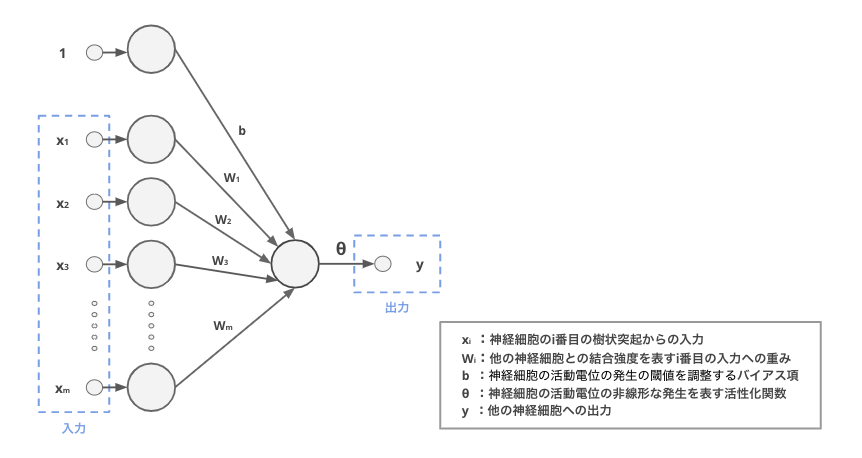
\includegraphics[width=0.5\columnwidth]{figure/neuron.png}
\caption[MLPの人工ニューロン]{人工ニューロン}
\label{fig:neuron}
\end{figure}

この時、他の神経細胞への出力$y$は、$x_i$の$W_i$を重みとした重み付き和に$b$を加えて活性化関数を作用させた値である。したがって、MLPの人工ニューロンは\prettyref{eq:MLP0_0}として定式化される。
\begin{align}
    \label{eq:MLP0_0}
    y=\theta(\sum_{i=1}^{m} W_{i} \times x_i+b)
\end{align}

\subsection{MLPの構造}

MLPは、\prettyref{fig:neuron}の人工ニューロンが複数並んだ層を一層とし(\prettyref{fig:MLP_net0})~、順伝播型の階層構造のニューラルネットワークを形成する~(\prettyref{fig:MLP_net1})~。また、入力層と中間層と出力層の三つの層構造を持ち、入力層と出力層はそれぞれ一層のみである。ここで、層を構成する人工ニューロンの全ての出力が次の層の全ての人工ニューロンの入力として渡されるため、MLPを構成する層を全結合層と呼ぶ。

\begin{figure}[b]
\centering
\begin{minipage}[b]{0.48\columnwidth}
\centering
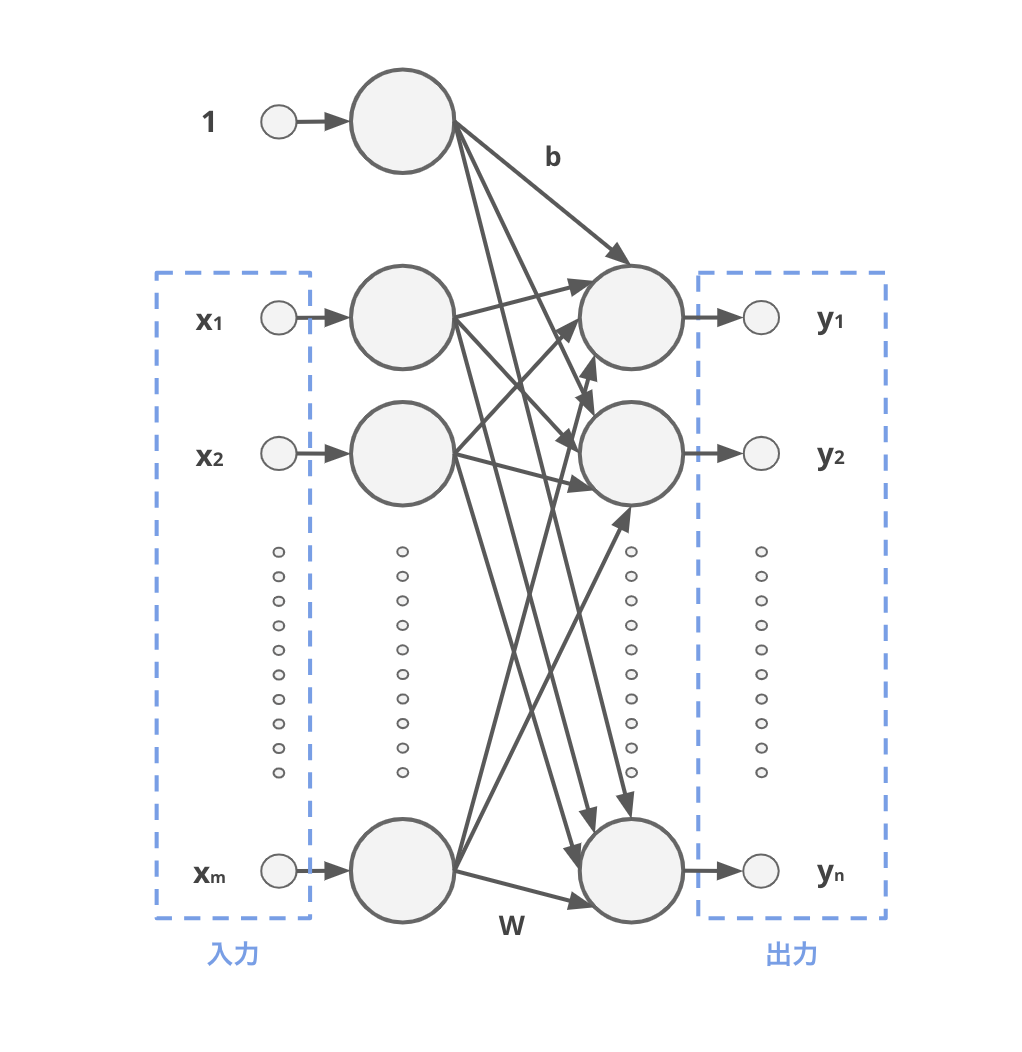
\includegraphics[width=0.8\columnwidth]{figure/mlp_net0.png}
\subcaption{MLPの一層}
\label{fig:MLP_net0}
\end{minipage}
\begin{minipage}[b]{0.48\columnwidth}
\centering
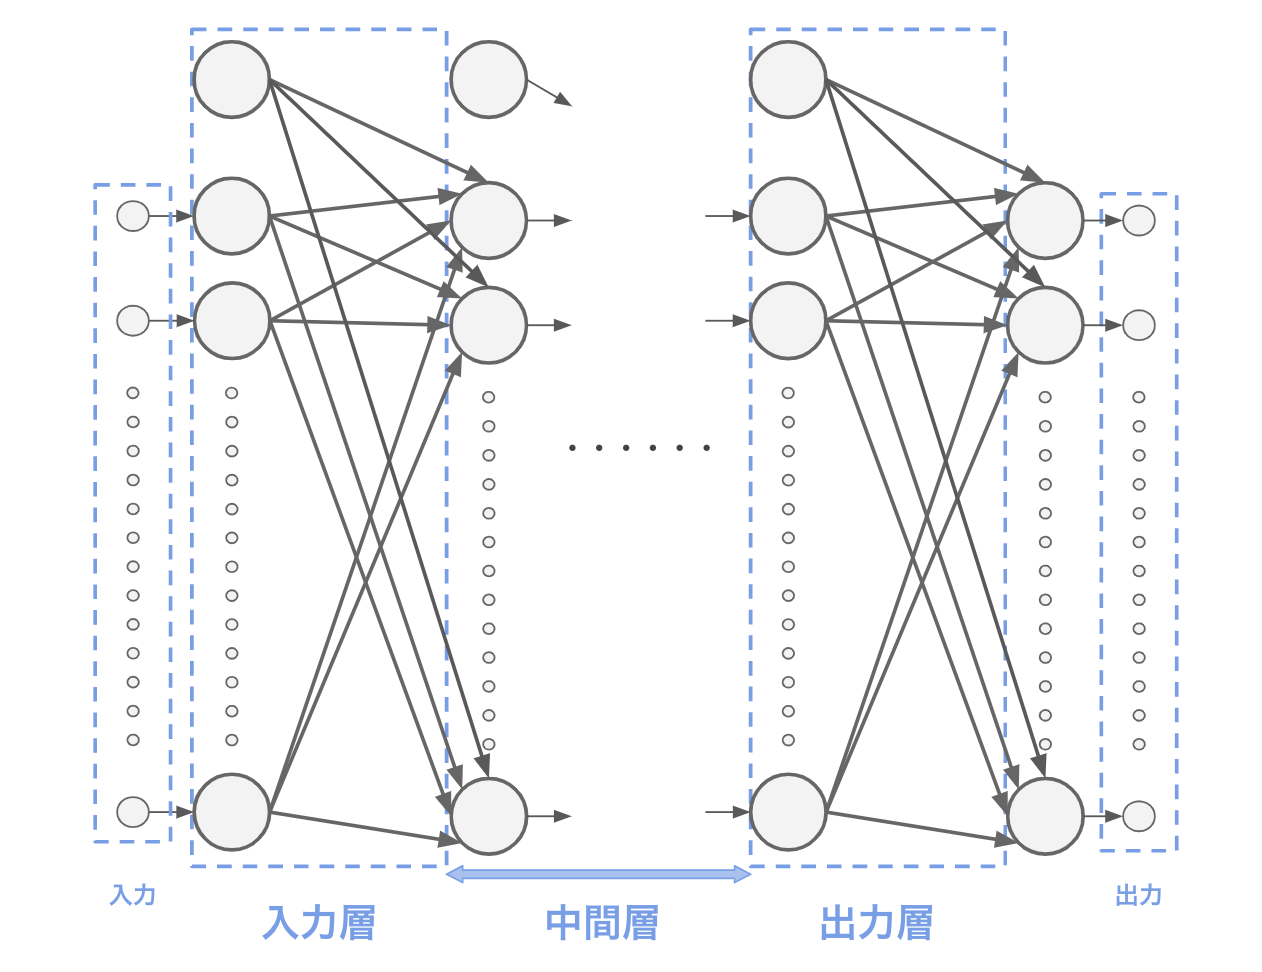
\includegraphics[width=\columnwidth]{figure/mlp_net1.png}
\subcaption{MLPの全層}
\label{fig:MLP_net1}
\end{minipage}
\caption{MLPのネットワーク}
\end{figure}

\subsection{MLPの定式化}

\prettyref{eq:MLP0_0}より一層の$j$番目の人工ニューロンの出力は\prettyref{eq:MLP0_1}となる。したがって、入力と出力とバイアス項をそれぞれベクトル$\boldsymbol{x},\boldsymbol{y},\boldsymbol{b}$で表し、重みを行列$W$で表すことで、MLPの一層の出力は\prettyref{eq:MLP0_2}と求まる。また、MLPは全結合層のみで構成されるため、何番目の層であるかを下付きの数字で表すことで、$n$層のMLPは\prettyref{eq:MLP0_3}として定式化される。
\begin{align}
    \label{eq:MLP0_1}
    y_j&=\theta(\sum_{i=1}^{m} W_{ji} \times x_i+b)\\
    \label{eq:MLP0_2}
    \boldsymbol{y}&=\theta(W\boldsymbol{x}+\boldsymbol{b})\\[8pt]
    \label{eq:MLP0_3}
    \boldsymbol{y}&=\theta_{n}(W_{n}(\theta_{n-1}(W_{n-1}\cdots(\theta_{1}(W_{1}\boldsymbol{x}+\boldsymbol{b_{1}}))\cdots+\boldsymbol{b_{n-1}}))+\boldsymbol{b_{n}})
\end{align}

\subsection{MLPの学習}

MLPでは実行可能解であるパラメータ$W_i,\boldsymbol{b_i}$の更新を繰り返すことで最適解を求める。この時、損失関数$L$の勾配を用いた最適化アルゴリズムである勾配降下法~\cite{GradientDescent}を用いて更新するのが一般的である。また、本節の手法は次章以降のCNNなどの他のニューラルネットワークにおいても用いられる。

\subsubsection{勾配降下法}
\label{sec:grad}

勾配降下法の中で単純なアルゴリズムである最急降下法を紹介する。最急降下法では、最も急な降下方向である勾配の反対方向へパラメータの更新を行うため、\prettyref{eq:MLP2_0}として定式化される。
\begin{align}
    \label{eq:MLP2_0}
    W _i , \boldsymbol{b _i} \leftarrow W_i - \eta \frac{\partial L}{\partial W_i} , \boldsymbol{b_i} - \eta \frac{\partial L}{\partial \boldsymbol{b_i}}
\end{align}

ここで、$\eta$は学習率と呼ばれる正の実数であり、更新の程度を指定する。また、本研究では勾配降下法としてAdam~\cite{Adam}を用いるため、その挙動を\prettyref{app:Adam}に示す。

\subsubsection{誤差逆伝播法}

勾配降下法ではそれぞれのパラメータにおいて損失関数の勾配を求める必要があり、高速に勾配を求める手法として誤差逆伝播法が一般に用いられる。また、誤差逆伝播法は大きく二つの段階に分けることができる。一つ目の段階では、与えられた学習データを元に入力層から出力層の方向にそれぞれの人工ニューロンの出力を求める。二つ目の段階では、出力層における損失関数の勾配を求めた後、勾配を誤差として出力層から入力層の方向に伝えつつ連鎖律を使用した勾配の計算をそれぞれのパラメータについて行う。また、誤差逆伝播法と連鎖律ついてはそれぞれ~\cite{Bishop}の5.3節と~\cite{Calculus}の4.4節に詳しい。

\subsubsection{バッチ処理}

\prettyref{sec:grad}で紹介した最急降下法では、パラメータの更新のたびに全ての学習データの期待値として誤差関数の値を計算する。このように全てのデータをひとまとめに扱う手法をバッチ処理と呼び、並列計算による高速化を行うことができる。しかし、パラメータの更新のたびに全データを扱うために、時間計算量と空間計算量のいずれも悪い手法となる。そこで、ミニバッチ処理と呼ばれる手法を用いるのが一般的である。ミニバッチ処理では、パラメータの更新のたびに指定したサイズ~(バッチサイズ)~のサブセットのみを用いる。これにより、時間計算量と空間計算量のいずれも改善しつつ並列計算による高速化を享受することができる。

%ここで改ページ
\clearpage

\section{CNN}

CNN~(Convolution~Neural~Network)~は、全結合層だけでなく畳み込み層とプーリング層を用いた順伝播型のニューラルネットワークである。2012年のILSVRCで2位以下に10\%以上の画像の認識精度の差をつけて優勝したAlexNet~\cite{AlexNet}はその著名な例である。また、本章では二次元データの画像でのCNNの説明を行うが、CNNについて詳しくは~\cite{CNN_recent}を参考にされたい。

\subsection{CNNと視覚野の関係}

CNNは脳の視覚野の機能を模倣するニューラルネットワークであり、Neocognitron~\cite{neocognitron}を起源に持つ。また、脳の視覚野には主に二つの機能がある。一つ目は刺激の位置により異なった位置のニューロンの活動電位を発生させることであり、二つ目は視覚情報の特徴を段階的に受容することである。

畳み込み層とプーリング層を用いることで二つの機能をCNNは表現する。まず、畳み込み層とプーリング層のいずれも局所領域間の位置関係を変えないため、前者の機能を模倣する。そして、畳み込み層では局所領域の特徴を抽出し、プーリング層では局所領域の特徴を集約するため、後者の機能を模倣する。

%畳み込み層では、人工ニューロン間の結合を局所領域に限定することで局所領域の特徴を抽出する。また、局所領域間の位置関係は変わらないため、前者の機能を模倣する。そして、プーリング層では、局所領域の人工ニューロンの出力をまとめることで局所領域の特徴を集約する。また、層を進むにつれて高段階の特徴が残るため、後者の機能を模倣する。

\subsection{CNNの畳み込み層}

畳み込み層では、カーネルと呼ばれるフィルターを用いて入力の行列に畳み込み演算を行い、行列を出力する~(\prettyref{fig:conv})~。カーネルは重みを成分に持つ行列であり、ストライドと呼ばれる一定の間隔を空けながら入力の行列の上を上下にスライドする。また、畳み込み演算ではカーネルにより覆われた入力の部分行列とカーネルとの間の内積を求める計算が行われる。そして、入力と出力の大きさを変えないために入力の周りに適当な幅で値を埋めるのが一般的であり、この操作をパディングと呼ぶ。

ここで、畳み込み層の入出力となる行列のことを特徴量マップと呼び、特徴量マップの枚数を表現する際には特徴量マップをチャンネルと呼ぶ。また、\prettyref{fig:conv}の畳み込み層は入力と出力として1チャンネルずつ持つが、入力と出力のいずれも複数チャンネルを取ることも可能である。そして、入力が複数チャンネルの場合はそれぞれの入力から求まる特徴量マップを成分ごとに足しあわせた結果が出力となり、出力が複数チャンネルの場合は1チャンネルの入力に対してカーネルが出力の数だけ必要となる。

\subsection{CNNのプーリング層}

プーリング層では、入力を局所領域に分解した後にそれぞれの領域への操作により情報量の圧縮を行う~(\prettyref{fig:pooling})~。また、この操作で最大値をとる場合をMax~Pooling、平均値をとる場合をAverage~Poolingと呼び、主にこの二つがプーリング層では用いられる。

\begin{figure}[b]
\centering
\begin{minipage}[b]{0.48\columnwidth}
\centering
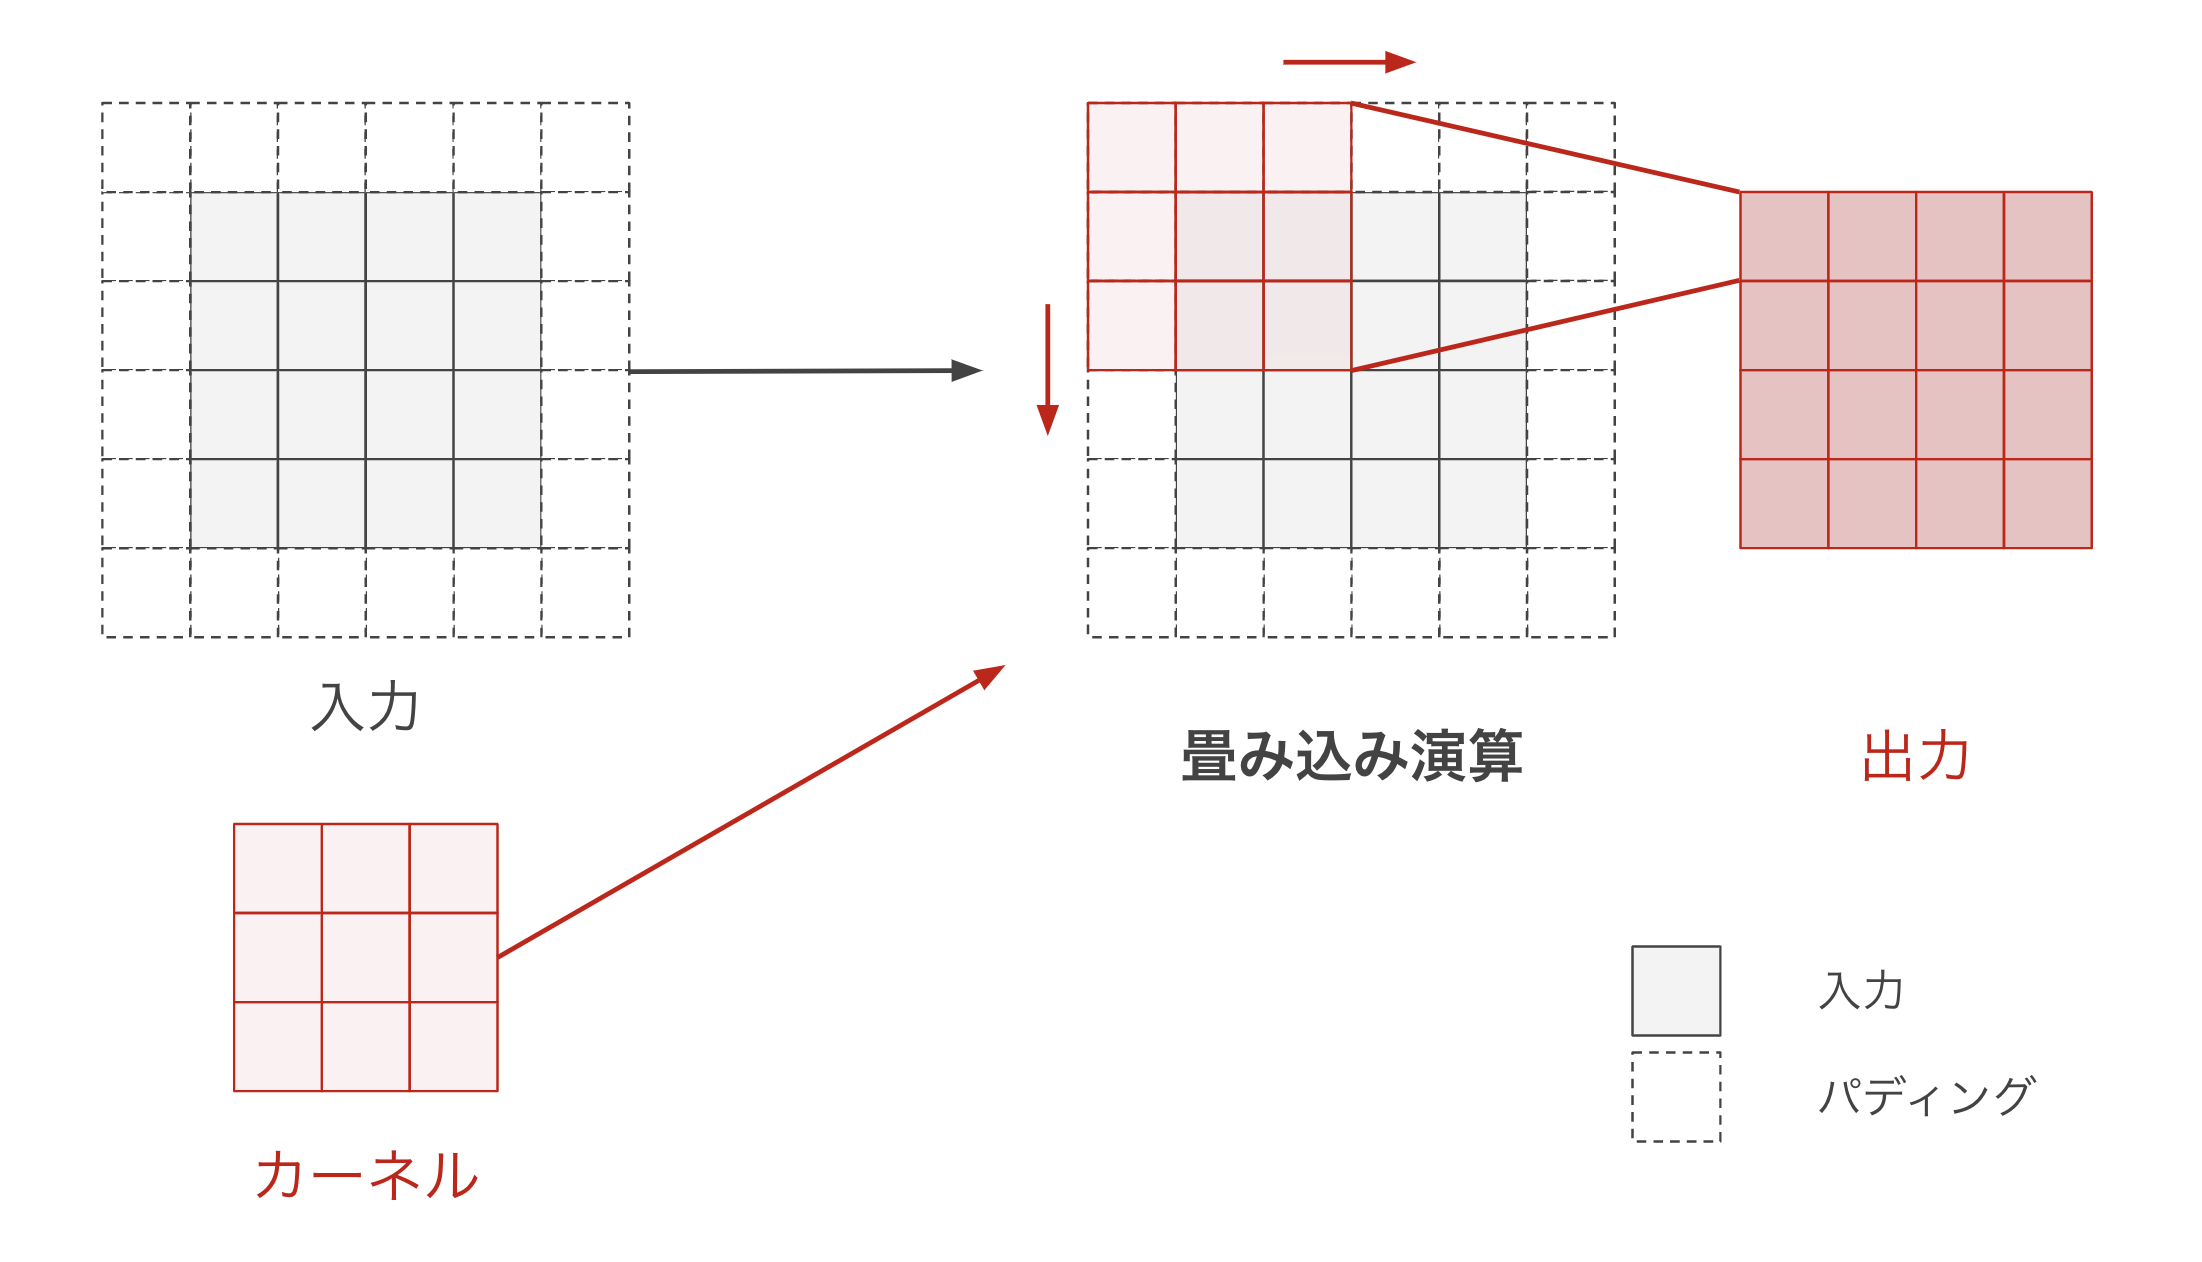
\includegraphics[width=0.9\columnwidth]{figure/convolution.png}
\caption[CNNの畳み込み層]{畳み込み層}
\label{fig:conv}
\end{minipage}
\begin{minipage}[b]{0.48\columnwidth}
\centering
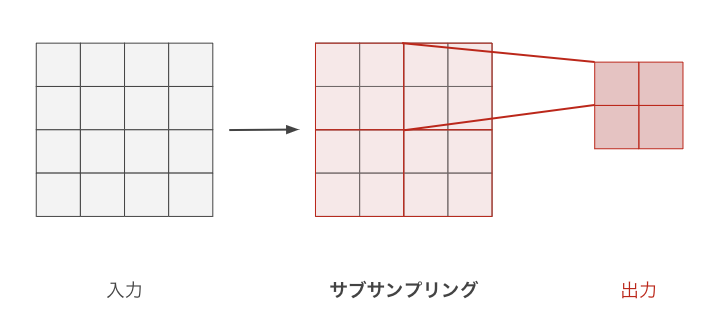
\includegraphics[width=\columnwidth]{figure/pooling.png}
\caption[CNNのプーリング層]{プーリング層}
\label{fig:pooling}
\end{minipage}
\end{figure}

%ここで改ページ
\clearpage

\section{GAN}

GAN~(Generative~Adversarial~Networks)~\cite{GAN}はニューラルネットワークの応用例であり、学習データの特徴を持つ擬似的なデータを生成することを目指す手法である。また、この手法を用いたDCGAN~\cite{DCGAN}のように、実在しない人やホテルの画像などを生成することも可能である。

\subsection{GANの概要}

GANはDiscriminator~(識別モデル)~とGenerator~(生成モデル)~の二つのニューラルネットワークにより構成される~(\prettyref{fig:GAN_net})~。まず、識別モデルはデータがFake~data~(生成モデルの出力)~とReal~data~(学習データ)~のどちらであるかを識別することを目標に学習を進める。そして、生成モデルは識別モデルが学習データであると誤って識別するほど学習データに近いデータを出力することを目標に学習を進める。この二つのモデルが競合的に学習を進めてナッシュ均衡の状態を目指すことで、漸進的に生成モデルが学習データにより近いデータを生成できるようになると期待される。また、生成モデルの入力には適当な次元のベクトルをノイズとして与えるのが一般的であり、ノイズは生成モデルの出力の揺らぎを表現する潜在変数の役割を担う。

\subsection{GANの定式化}

GANでは、生成モデルと識別モデルの目的関数をそれぞれ\prettyref{eq:GAN_G}、\prettyref{eq:GAN_D}として定式化する。また、学習データを$\boldsymbol{x}$、生成モデルの出力を$G(\boldsymbol{z};\theta_G)$、ノイズを$\boldsymbol{z}$、識別モデルの出力を$D(\cdot;\theta_D)$、生成モデルと識別モデルのパラメータをそれぞれ$\theta_G,\theta_D$、とする。
\begin{align}
    \label{eq:GAN_G}
    \argmin _{\theta_G}& \mathbb{E}_{\boldsymbol{z}}[\log (1-D(G(\boldsymbol{z};\theta_G);\theta_D))]\\
    \label{eq:GAN_D}
    \argmax _{\theta_D}& \mathbb{E}_{\boldsymbol{x}}[\log D(\boldsymbol{x};\theta_D)]+\mathbb{E}_{\boldsymbol{z}}[\log (1-D(G(\boldsymbol{z};\theta_G);\theta_D))]
\end{align}

\begin{figure}[b]
\centering
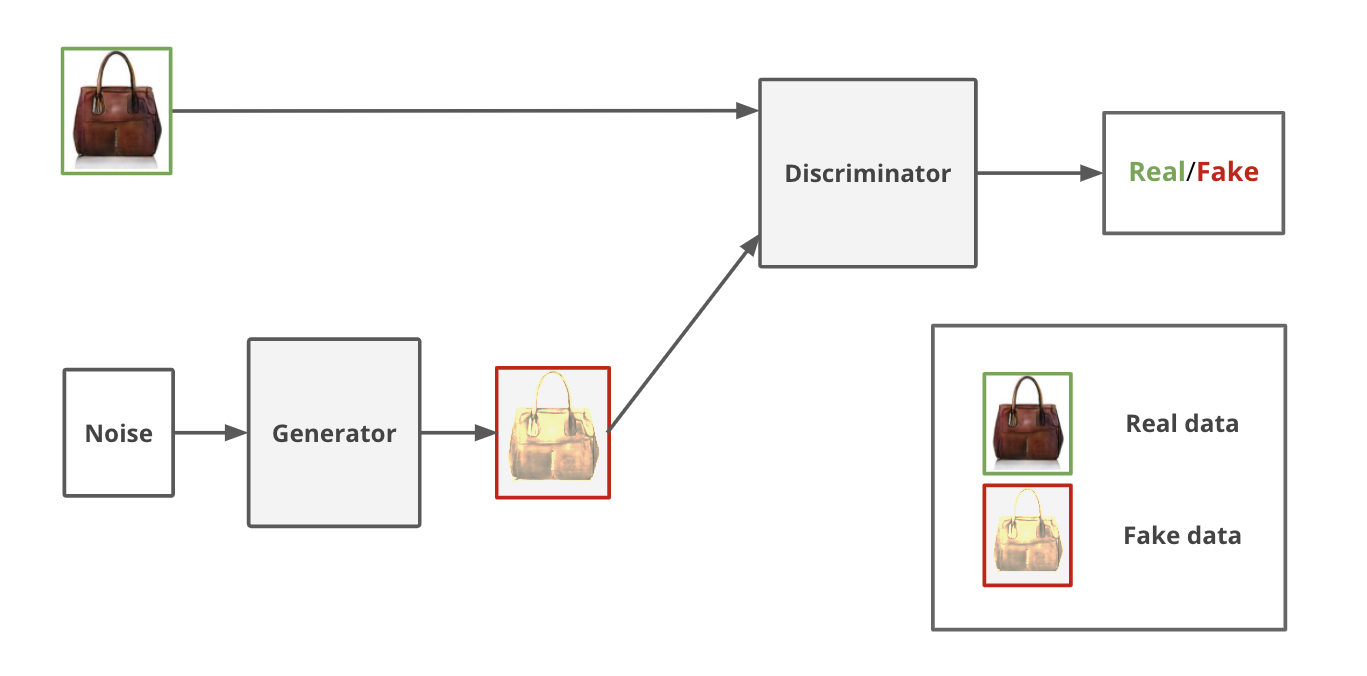
\includegraphics[width=0.9\columnwidth]{figure/GAN_net.png}
\caption{GANの全体図}
\label{fig:GAN_net}
\end{figure}

%ここで改ページ
\clearpage

\section{Pix2pix}

Pix2pix~\cite{pix2pix}は生成モデルと識別モデルのいずれにも変換元の画像を条件として与えることで画像の変換を行うGANである~(\prettyref{fig:pix2pix_net})~。具体的には、線画から写真への変換~(\prettyref{fig:pix2pix_img1})~や白黒画像からカラー画像への変換~(\prettyref{fig:pix2pix_img2})~を行うことができる。

\begin{figure}[b]
\centering
\begin{minipage}[b]{0.48\columnwidth}
\centering
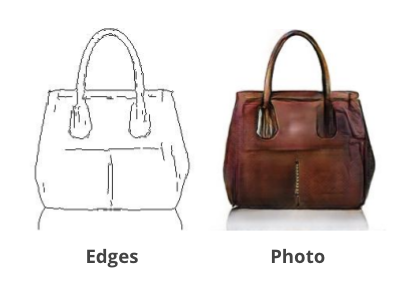
\includegraphics[width=0.8\columnwidth]{figure/EP.png}
\subcaption{Edges~to~Photo}
\label{fig:pix2pix_img1}
\end{minipage}
\begin{minipage}[b]{0.48\columnwidth}
\centering
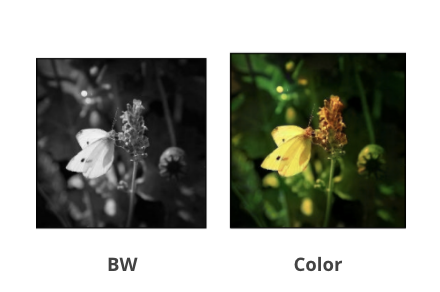
\includegraphics[width=0.8\columnwidth]{figure/BWC.png}
\subcaption{BW~to~Color}
\label{fig:pix2pix_img2}
\end{minipage}
\caption{Pix2pixのスタイル変換の例}
\label{fig:pix2pix_img}
\end{figure}

\begin{figure}[b]
\centering
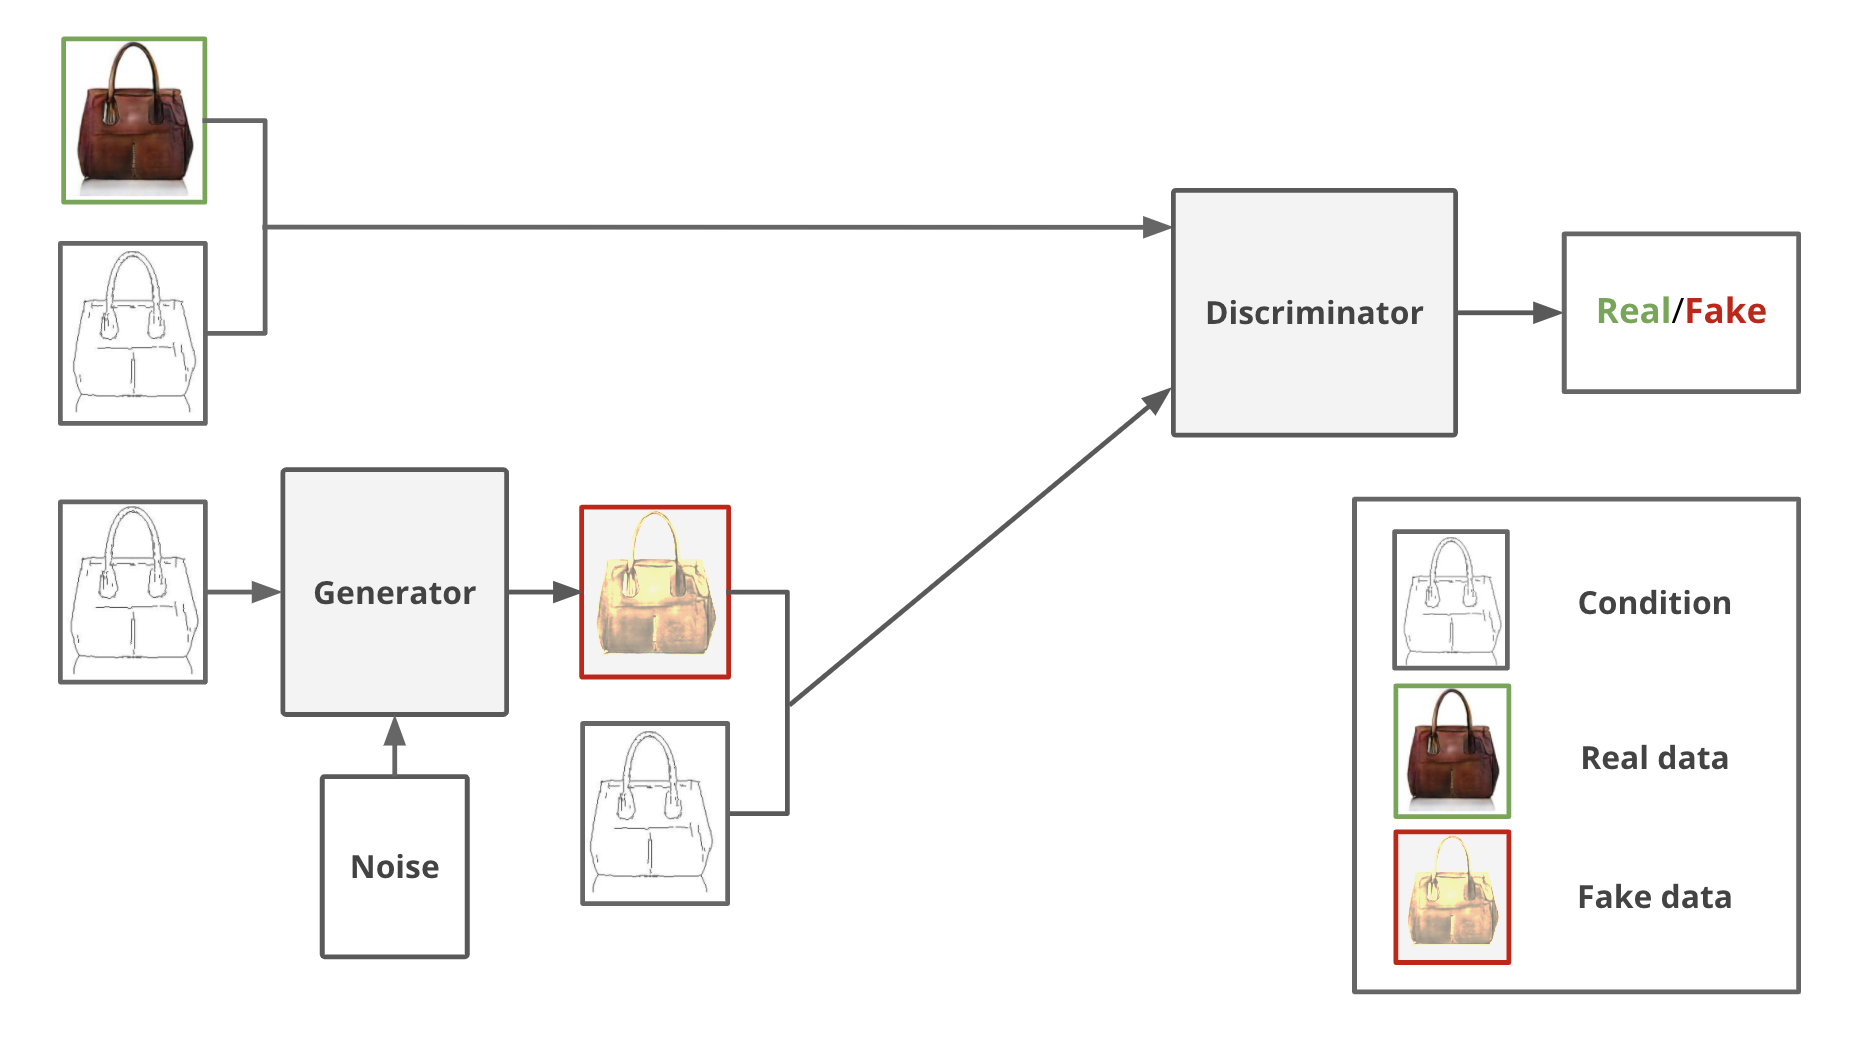
\includegraphics[width=0.9\columnwidth]{figure/pix2pix_net.png}
\caption{Pix2pixの全体図}
\label{fig:pix2pix_net}
\end{figure}

\subsection{Pix2pixの定式化}

Pix2pixでは、生成モデルと識別モデルの目的関数をそれぞれ\prettyref{eq:pix2pix_G}、\prettyref{eq:pix2pix_D}として定式化する。また、目的関数はGANとほとんど同じであるが、変換元の学習データ$\boldsymbol{y}$を条件として与える点と生成モデルの目的関数に変換先の学習データと生成モデルの出力の差分のL1ノルムを含める点が異なる。
\begin{align}
    \label{eq:pix2pix_G}
    \argmin _{\theta_G}& \mathbb{E}_{\boldsymbol{y}, \boldsymbol{z}}[\log (1-D(\boldsymbol{y}, G(\boldsymbol{y}, \boldsymbol{z}; \theta_G); \theta_D))]+\lambda \mathbb{E}_{\boldsymbol{x}, \boldsymbol{y}, \boldsymbol{z}}[\|\boldsymbol{x}-G(\boldsymbol{y}, \boldsymbol{z}; \theta_G)\|_{1}]\\
    \label{eq:pix2pix_D}
    \argmax _{\theta_D}& \mathbb{E}_{\boldsymbol{x}, \boldsymbol{y}}[\log D(\boldsymbol{y}, \boldsymbol{x}; \theta_D)]+\mathbb{E}_{\boldsymbol{y}, \boldsymbol{z}}[\log (1-D(\boldsymbol{y}, G(\boldsymbol{y}, \boldsymbol{z}; \theta_G); \theta_D))]
\end{align}

%ここで改行
\clearpage

\subsection{Pix2pixの生成モデル}

Pix2pixの生成モデルには、スキップコネクションを持ったEncoder-Decoderを用いる~(\prettyref{fig:u-net})~。また、Dropout層によりGANのノイズを表現する。ここで、Dropout~\cite{Dropout}とは学習時にベルヌーイ分布に従ってランダムにある層の重みの一部を0として無視する正則化の手法である。

\subsubsection{Encoder-Decoder}

Encoder-Decoderは、画像から特徴量を抽出する処理~(Encode)~と特徴量を元に画像を再構成する処理~(Decode)~の二段階で構成されたモデルである。また、Pix2pixでは、Encodeの部分に畳み込み層を用い、Decodeの部分に逆畳み込み層を用いる。逆畳み込み層は畳み込み層の逆演算に相当する演算を行う層であり、~\cite{Deconv}の3.2.2節に詳しい。

\subsubsection{スキップコネクション}

Pix2pixの生成モデルは\prettyref{fig:u-net}で表現されるスキップコネクションを持つ。このスキップコネクションはU-net~\cite{u-net}由来のものであり、変換前後の画像でのピクセルの対応関係を維持する役割を担う。

\subsection{Pix2pixの識別モデル}

Pix2pixの識別モデルでは、CNNを用いてパッチと呼ばれる小領域ごとに真偽を求め、その平均を出力とする~(\prettyref{fig:patchgan})~。また、Pix2pixではこの識別モデルをPatchGANと名付けた。

\begin{figure}[b]
\centering
\begin{minipage}[b]{0.52\columnwidth}
\centering
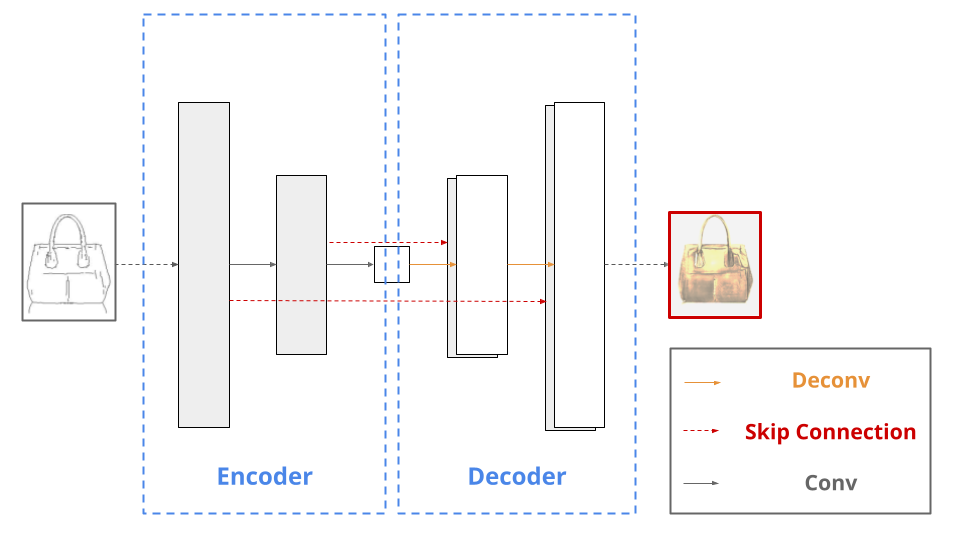
\includegraphics[width=\columnwidth]{figure/u-net.png}
\subcaption[Pix2pixの生成モデル]{生成モデルのネットワーク}
\label{fig:u-net}
\end{minipage}\\
\begin{minipage}[b]{0.52\columnwidth}
\centering
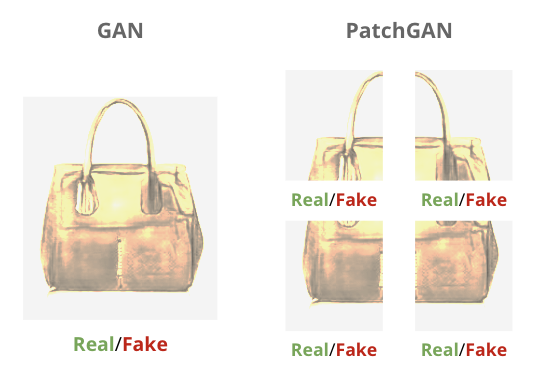
\includegraphics[width=\columnwidth]{figure/patchgan.png}
\subcaption{GANとPatchGANの識別モデルの比較}
\label{fig:patchgan}
\end{minipage}
\caption[Pix2pixの生成モデルと識別モデル]{}
\end{figure}